\chapter{Medical background}

\section{Human teeth}
Human dentition is composed of two sets of teeth - primary and permanent. The primary, also called deciduous, consists of 20 teeth and begins to erupt at 6 months of age. This dentition is completely replaced at the approximate age of 13 years by permanent teeth consisting of 32 teeth. These can be divided into 4 classes on the basis of function and form. Namely, those classes are:

\subsubsection*{Incisors}
A total of 8 incisors teeth are found in primary and permanent dentition. They are located at the oral cavity entrance, and their main purpose is to cut and shear food. They are essential for the esthetics of a smile and also play a vital role in phonetics.

\subsubsection*{Canines}
Canines, at a total number of 4, are located at the corner of dental arches creating dividing it to a frontal and a lateral part. They have a triangular shape with a single cusp tip on the incisal edge. The structure is associated with their ability to seize, pierce, tear and cut food. Along with the incisors, they are important for esthetics.

\subsubsection*{Premolars}
Premolars are teeth found only in permanent dentition, being the successional teeth of all primary 8 molars. Premolars share functional characteristics of canines and molars - they both seize and grind food thanks due to their anatomy.

\subsubsection*{Molars}
Human dentition contains 12 molars with no deciduous predecessors. Their main role is crushing and grinding food to dimensions appropriate for swallowing. Broad occlusal surfaces make them capable of this task. Molars are prone to dental caries due to the presence of deep grooves that run across the occlusal surface of the teeth and wide area of contact between adjacent molars. Both of these places are difficult to clean, resulting in a space where bacterias tend to accumulate.


\subsection{Structure of teeth}
Teeth are composed of three structures: Enamel, pulp-denting complex and cementum. A picture of teeth structure is depicted in the figure

\subsection*{Enamel}
The superficial layer covering the anatomic crown of a tooth consists of a highly mineralized crystalline structure called the enamel. More than 90\% of the volume is taken up by minerals (hydroxyapatite), making enamel the hardest substance of teeth and even the human body. Its thickness varies from one class of tooth to another, but it ranges from 2 to 3mm on average. Enamel is produced in the process of amelogenesis by ameloblast cells occuring only in the development stage. Hence it does not have the ability of regeneration. The biggest threat to enamel are acidic conditions, which can cause its dissolution. This causes enamel to demineralize, and when the cause is not removed, the enamel starts to cavitate irreversibly. Enamel has the ability to remineralize.

\subsection*{Pulp-Dentin complex}
Pulp and dentin are two specialized connective tissues, however by some sources are considered to be a single tissue forming a complex.
The dental pulp is located in the pulp cavity of the tooth, and it serves four functions: formative, nutritive, sensory and reparative.
The pulp is circumscribed by dentin formed by cells called odontoblasts in the process of dentinogenesis. Their cell bodies are located in the pulp cavity, but their cytoplasmic cell processes, located in dentinal tubules, extent into the mineralized dentin. Thanks to those processes, dentin is considered to be a living tissue. Its function is to provide the ability to regenerate and react to pathological stimuli, such as blocking the advancement of carious lesions by precipitating minerals in the affected area.
Dentin forms the largest portion of the tooth. In the coronal part, it is covered by the enamel and by cementum on the anatomic root of the tooth. There are different types of dentin.
\begin{itemize}
    \item \textbf{Primary dentin} forms the outer and largest layer of dentin closest to the enamel. It is produced in the development stage of the tooth.
    \item \textbf {Secondary dentin} is formed after the tooth is erupted and functional.
    \item \textbf{Tertiary reactive dentin} production is encouraged as a response to pathological stimuli, such as injury or caries. It is produced at the pulp-dentine interface in order to protect the pulp.
    \item \textbf{Transparent dentin} results from physical occlusion of dentinal tubules leading to an increase in transparency.
\end{itemize}


\subsection*{Cementum}
Cementum covers the anatomic roots of teeth. Its structure consists of approximately 50 \% of anorganic material and 50 \% of organic matter and water, making it slightly softer than dentin and far softer than enamel. It plays a role in attaching the tooth to the alveolus. Cementum possesses the ability to repair itself to a limited degree.

\section{Dental caries}

\subsection{Cause}
Dental caries is a preventable chronic and biofilm-mediated disease. The main cause is dental plaque (also called biofilm). Plaque is composed of bacteria, their by-products and water and has the ability to adhere to the tooth structure. Some bacteria in the plaque metabolize refined dietary carbohydrates and produce organic acid by-products. Those acids, if present in the biofilm for an extended period of time, can lower the PH in the biofilm to below a critical threshold (5.5 for enamel, 6.2 for dentin). Low pH drives phosphate and calcium from the tooth into the biofilm in attempt to reach an equilibrium. This loss of minerals in tooth is called demineralization and if not stopped can lead to a caries lesion. However, this process can be stopped and eventually reverted if the pH returns to neutral and the relative concentration of soluble calcium and phosphate in the biofilm is higher than in the tooth. This process occurs multiple times a day and are modulated by many factors that are highly individual and tooth specific. They will differ from person to person.


\subsection{Classification of dental caries}
Dental caries are classified on multiple bases. The common ones are: Depth of the lesion or lesion activity. \newline
A frequently used classification scheme was proposed by Pitts \& Fyffe in 1988 including a total of 4 categories, three for cavitated lesions and one for non-cavitated lesions.
\begin{itemize}
    \item \textbf{D0} Surface sound. No evidence of either treated and untreated caries.
    \item \textbf{D1} Initial Caries. No detectable loss of tooth substance. Staining in fissures or rough spots in enamel may be visible, but these spots do not catch the explorer.
    \item \textbf{D2} Enamel caries. Demonstrable loss of tooth substance. Chalky or crumbled texture of the material within the cavity. No evidence, that cavitation has penetrated through the enamel layer into the dentin.
    \item \textbf{D3} Caries of dentin. The floor or wall of the cavity is softened. The tip of the explorer must enter a lesion with certainty.
    \item \textbf{D4} Pulpal involvement. Deep cavity with probable involvement of the pulp. A probe should not be used to probe the pulp.
\end{itemize}

\subsection{Diagnosis}
Visual-tactile diagnosis is the primary way to inspect teeth and detect caries. Dentists use a mouth mirror and sharp probe to perform the examination. It is vital to dry teeth since the difference in the refractive index between sound and carious enamel is higher when water is removed from the tissue. This increases the chance of spotting a carious lesion before it has a chance to progress and cavitate the tooth.
The second most used method used by clinicians to complement the visual examination is a dental X-ray. In dentistry there are 2 main types of X - ray imaging taken during the examination: intraoral (the X-ray film is located inside the mouth) and extraoral (the X-ray film is outside the mouth). The intraoral images are the most commonly taken ones. This cathegory include bitewing and periapical X-rays among others, each featuring different aspects of the teeth. The extraoral imaging is mostly used to detect any dental problems located in the jaw and skull area. The most common one to be used is a panoramic radiograph.

\newline
Less common diagnostic measures are:
\begin{itemize}
    \item Laser light-induced fluorescence
    \item Digital imaging fiber-optic transillumination
    \item Electrical conductance and impedance measurement
\end{itemize}

\subsubsection{Bitewing X-ray}
The bitewing radiograph is an image that depicts the upper and lower teeth in one region of the mouth as seen in figure \ref{fig:bitewing_sample}. It gives a clear sight of the interproximal surfaces allowing good caries detection in this area. Interproximal caries are difficult to diagnose by the visual-tactile method, thus using the bitewing X-ray can lead to an early diagnosis and a chance for the enamel to remineralize. Also, it portrays the alveolar crest where any changes in thickness of the bone due to a periodontal disease may be noticed. Unlike the other intraoral method, it does not show the full length of the teeth. This type of dental X-ray is the most commonly taken one for preventive purposes. 

\subsubsection{Periapical X-ray} 
Periapical X-ray portraits the tooth from the crown to where the root attaches into the jaw, hence the whole length of a tooth is visible. It only shows the upper or lower teeth in one part of the jaw as portrayed in figure \ref{fig:periapical_sample}  Periapical X-ray allows to detect any abnormalities in the root and any periapical lesions.

\subsubsection{Panoramic X-ray}
This type of extraoral dental image shows the entire mouth area including the upper and lower jaw and adjacent structures. It depicts the fully emerged teeth along with the ones that are not fully erupted yet. Impacted teeth, i.e. wisdom teeth as seen in figure \ref{fig:panoramatic_xray}, can be identified as well.  Panoramic X-ray is often used before major procedures or to diagnose jaw tumors, cysts, fractures or sinusitis. Nevertheless, it is not usually taken in order to diagnose dental caries.

\subsubsection{Digital imaging fiber-optic transillumination (DIFOTI)}
DIFOTI is different from the previously mentioned types of dental imaging. Unlike the others, it works with an infrared fiber-optic light and not X-ray. The optical properties of a lesion are different than in  healthy dental tissue, therefore making it appear darker. DIFOTI enables the detection of fissure/occlusal caries, interproximal caries and fractures and cracks in the tooth. It is used as a noninvasive method since it does not expose the patient to ionizing radiation. 

\subsection{Treatment}
Based on the progression of the lesion and the patient's risk profile, treatment is suggested. In some cases, only instructions to increase oral hygiene together with fluoride toothpaste are enough to stop the progression and lead to remineralization of the enamel. The dentist can suggest application of a sealant to stop further progression of the lesion. If this treatment is perceived as insufficient given the mentioned factors, restoration of the tooth is required. This consists of the removal of all dental decay and filling the cavity with restorative material such as dental composite or amalgam.

\subsection{Epidemiology}
Untreated dental caries in permanent teeth is the most prevalent medical condition \cite{Kassebaum2015}. In 2010 around 35\% of the global population was affected. The biggest prevalence was observed around the age of 25. The sex of a person was not a significant factor in the statistics. No noticeable change in prevalence occurred between the years 1990 and 2010 \cite{Kassebaum2015} \cite{Frencken2017}, which means that the technological improvement in dentistry had no effect on the prevalence.
Kassenbaum et al. suggest that 42 new cases of tooth decay in primary and permanent teeth will develop annually from 100 people followed up. This imposes a burden on health care systems. According to Huang et al. \cite{Hung2020} in the United States alone, the cost of dental care in 2016 was 0.1 trillion \$ out of total health care expenditure of 1.62 trillion \$.

\begin{figure}
    \centering
    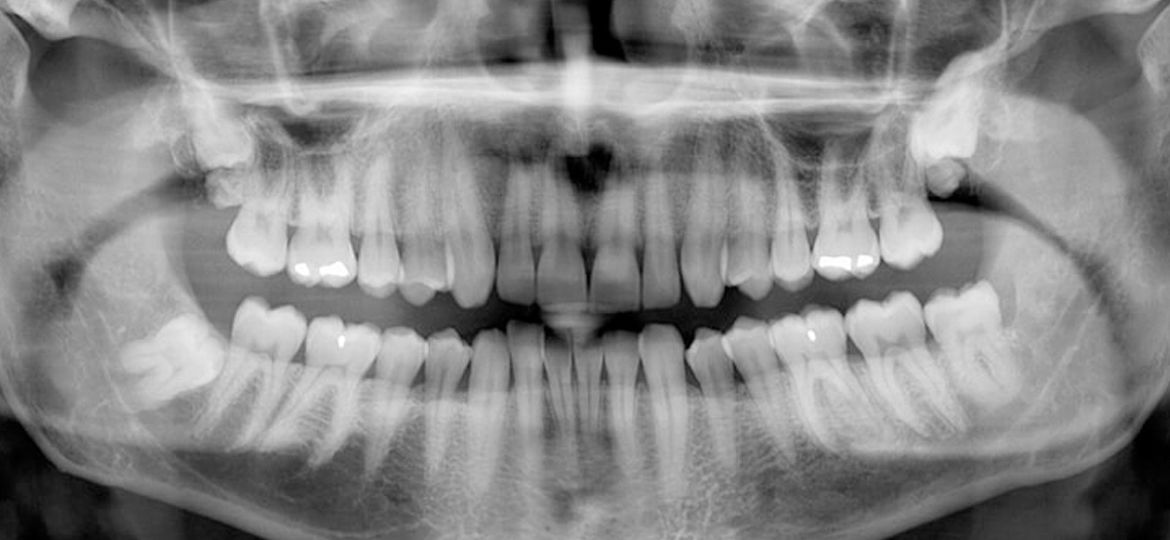
\includegraphics[width=\linewidth]{images/panoramatic_xray.jpg}
    \caption{Panoramatic X-ray image, source \cite{Panoramatic2017}}
    \label{fig:panoramatic_xray}
\end{figure}


\begin{figure}
    \begin{floatrow}[2]
        \ffigbox[\FBwidth]{\caption{Bitewing X-ray image}\label{fig:bitewing_sample}}%
        {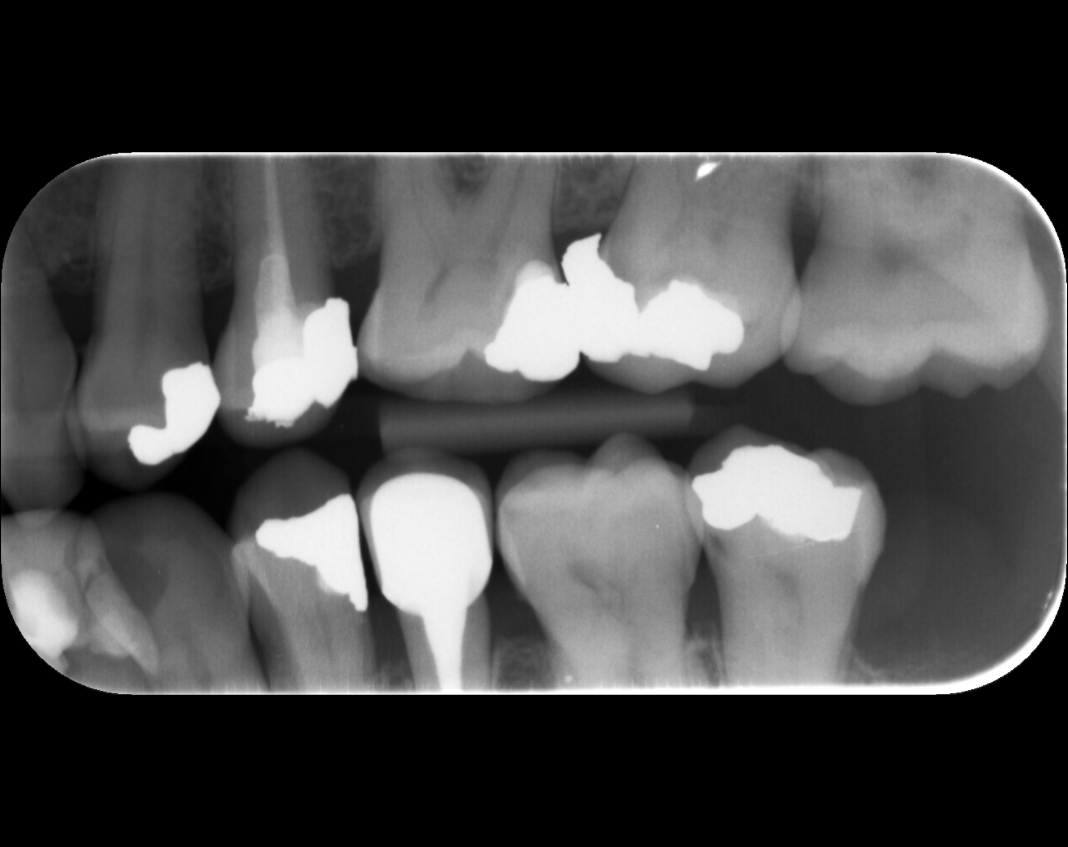
\includegraphics[width=\linewidth]{images/bitewing_xray.png}}\;
        \ffigbox[\FBwidth]{\caption{Periapical X-ray image, source \cite{Creanga2015}}\label{fig:periapical_sample}}%
        {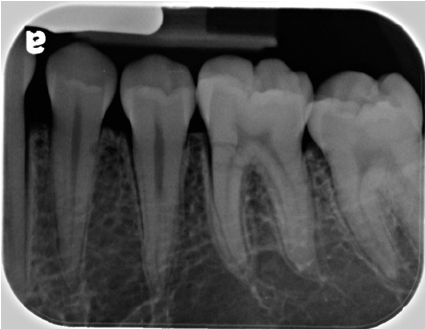
\includegraphics[width=\linewidth]{images/periapical_xray.png}}
    \end{floatrow}
\end{figure}